Here we compare projected statistical errors of a DES like survey 
to systematic errors introduced by shape measurement bias on 
a simulated stacked cluster weak lensing
analysis. The distribution of cluster properties that we use is 
expected to be comperable to the distribution of clusters that will
be observed by DES. The statistical error we model for the stacked
cluster mass is dominated by shape noise in the background galaxies
and is modeled using the formula described in \citep{obscos, mbecker}.
\indent To create a simulated DES like stacked weak lensing survey we
take a simulated halo distribution, and then bin by mass and
redshift. For an analysis on observed data the clusters would
be binned by observables that are correlated with cluster mass such as richness,
optical luminosity, and X-ray luminosity. The different mass proxies used will
scatter some clusters into bins with a different median mass, but
will hopefully not greatly effect the average shear profile. In this
study we divide the cluster sample into four mass bins and six
redshift bins. The average mass, concentration, and redshift of the
clusters in each bin is determined and then used to calculate the
expected statistical error and an average NFW shear profile.  The
number of clusters in each mass bin and thier average redshift is
shown in Figure \ref{fig:N_Halo}. \\  
\indent To estimate the average redshift of background galaxies behind
each bin 
we use a redshift distribution of galaxies expected by a DES like survey
\begin{equation}
f(z) = z^m exp(-( z/z_* )^{\beta}) 
\end{equation}
where $m=2.0 $, $z_*=0.5$ and $\beta = 2.0 $ as described in
\citep{obscos}. The average redshift of sources selected behind each
stacked weak lensing bin is shown in in Table
\ref{table:NWF_1_b} and Table \ref{table:NWF_4_b}.
\indent
The statistical error or mass uncertainty $\Delta$ ln$(M)$ as
described in \citet{obscos} for stacked weak lensing is :
\begin{equation}
\Delta \rm{ln}(M) = \sqrt{ (\Delta  \rm{ln} (M_{s}))^2 +
(\sigma_{wl} )^2 }
\end{equation}
which combines the error due to the shape noise and the error due to
scatter based on clusters not being spherical. From \citep{mbecker}
we take
\begin{equation}
\sigma_{wl} = \frac{0.3}{\sqrt{N}}
\end{equation}
where N is the number of clusters in a given bin. To calculate the
shape noise we use the equation
\begin{equation}
\Delta \rm{ln} (M_{s}) = 6.0*10^3
(\frac{N}{N_{A}})^{0.5} (\frac{M}{M_{o}})^{-0.66} (\frac{\overline{ngal}}{N_{o}})^{-0.5}(\frac{D_{A}}{0.5})^{-1}
\end{equation}
from \citep{obscos} . To model the concentration we expect
for clusters at this redshift we assign an initial concentration c
\begin{equation}
c= A*( m_{200}/(2.0*1.e12))^{B}*(1 + z_{\rm{cluster}})^{C}
\end{equation}
Where  $ A = 7.85 $ ,  $ B = -0.081 $ , $ C= -0.71 $ and $m_{200}$ is
the mass within $r_{200}$ from \citep{oguri}.

\begin{figure}
 \centering  % this centres figure in column
  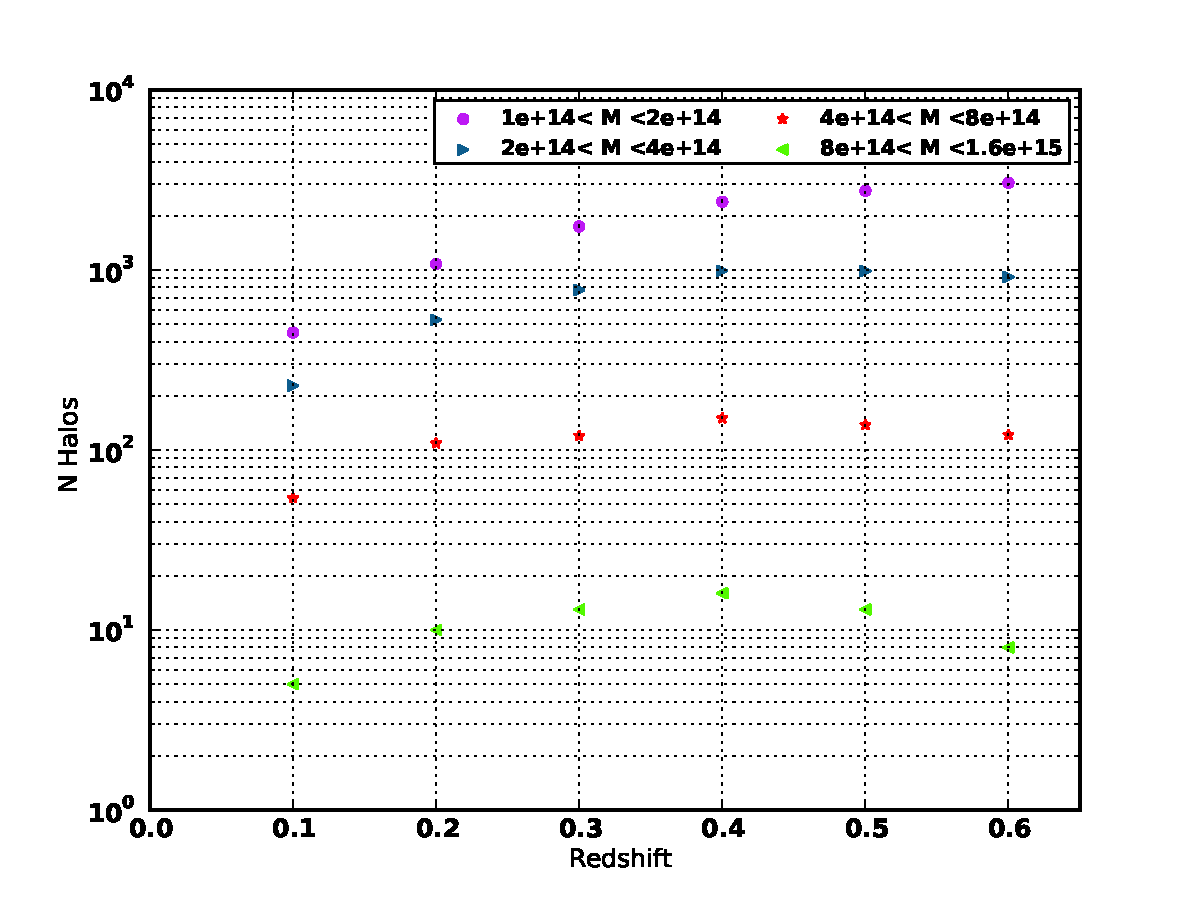
\includegraphics[width=0.55\textwidth]{fig/Halo_N.pdf} 
  \caption{The number of halos in each given mass bin.}
\label{fig:N_Halo}
\end{figure} 